\documentclass[12pt,a4paper]{article}
\usepackage[margin=1in]{geometry}
\usepackage[T1]{fontenc}
\usepackage{graphicx}
\usepackage{booktabs}
\usepackage{longtable}
\usepackage{array}
\usepackage{hyperref}
\usepackage{xcolor}
\usepackage{float}
\hypersetup{colorlinks=true,linkcolor=blue,urlcolor=blue,citecolor=blue}

\title{ImpactLedger: Corrected Implementation Report\\\large(Code-Grounded Revision of draft7)}
\author{Project Documentation Update}
\date{\today}

\begin{document}
\maketitle

\section*{Abstract}
This report replaces mismatched claims from the prior draft with statements grounded in the current repository implementation. The corrected system is a Next.js App Router application backed by Supabase/PostgreSQL, with role-aware modules for donor, volunteer, and organization-admin workflows. Donation flows are integrated with Razorpay checkout and webhook reconciliation, with invoice dispatch and receipt generation handled by server modules.

\section{Scope and Correction Strategy}
The objective is to align documentation with implemented behavior rather than preserve legacy assumptions. We used:
\begin{itemize}
  \item code inventory of pages, APIs, server modules, and schema;
  \item extracted claim clusters from \texttt{draft7.pdf};
  \item mismatch normalization into a claim-correction matrix.
\end{itemize}

The matrix source is provided in \texttt{report/claim\_mismatch\_matrix.csv}.

\section{Implemented Tech Stack}
\textbf{Frontend and runtime:}
\begin{itemize}
  \item Next.js + React (App Router).
  \item Route handlers under \texttt{src/app/api/**/route.ts}.
\end{itemize}

\textbf{Data and auth:}
\begin{itemize}
  \item Supabase/PostgreSQL schema in \texttt{supabase/schema.sql}.
  \item Supabase auth with tenant role resolution in \texttt{src/lib/server/auth.ts}.
\end{itemize}

\textbf{Payments and receipts:}
\begin{itemize}
  \item Razorpay order creation and signed webhook verification.
  \item Invoice dispatch via SMTP and generated receipt PDFs.
\end{itemize}

\textbf{Tooling scripts:}
\begin{itemize}
  \item \texttt{npm run lint}, \texttt{npm run test}, \texttt{npm run build}.
\end{itemize}

\section{Functional Scope (Implemented Features)}
\subsection{Public}
Campaign listing and details, donation entry points, transparency view, impact page, and policy/legal pages.

\subsection{Donor}
Dashboard and donation history endpoints/pages.

\subsection{Volunteer}
Dashboard, assignments, logs, resources, and verification pages with corresponding APIs.

\subsection{Organization Admin}
Dashboard, campaigns, donors, operations, reports, analytics, and settings APIs/pages.

\section{Route and API Surface}
The canonical route inventory is maintained in \texttt{report/canonical\_inventory.md}. In summary:
\begin{itemize}
  \item App pages are defined under \texttt{src/app/**/page.tsx}.
  \item APIs are defined under \texttt{src/app/api/**/route.ts}.
  \item Payment APIs include checkout, verification, Razorpay webhook; Stripe webhook endpoint remains but is explicitly deprecated with HTTP 410.
\end{itemize}

\section{Data Model}
The application uses a multi-tenant relational model in Supabase/PostgreSQL. Core domains include:
\begin{itemize}
  \item tenant and membership tables for RBAC;
  \item campaign, donor, donation, and financial ledger tables;
  \item volunteer profile/assignment/report tables;
  \item audit and webhook event logging tables;
  \item reporting views for campaign funding and transparency.
\end{itemize}

\section{Architecture and Design}
\begin{figure}[H]
  \centering
  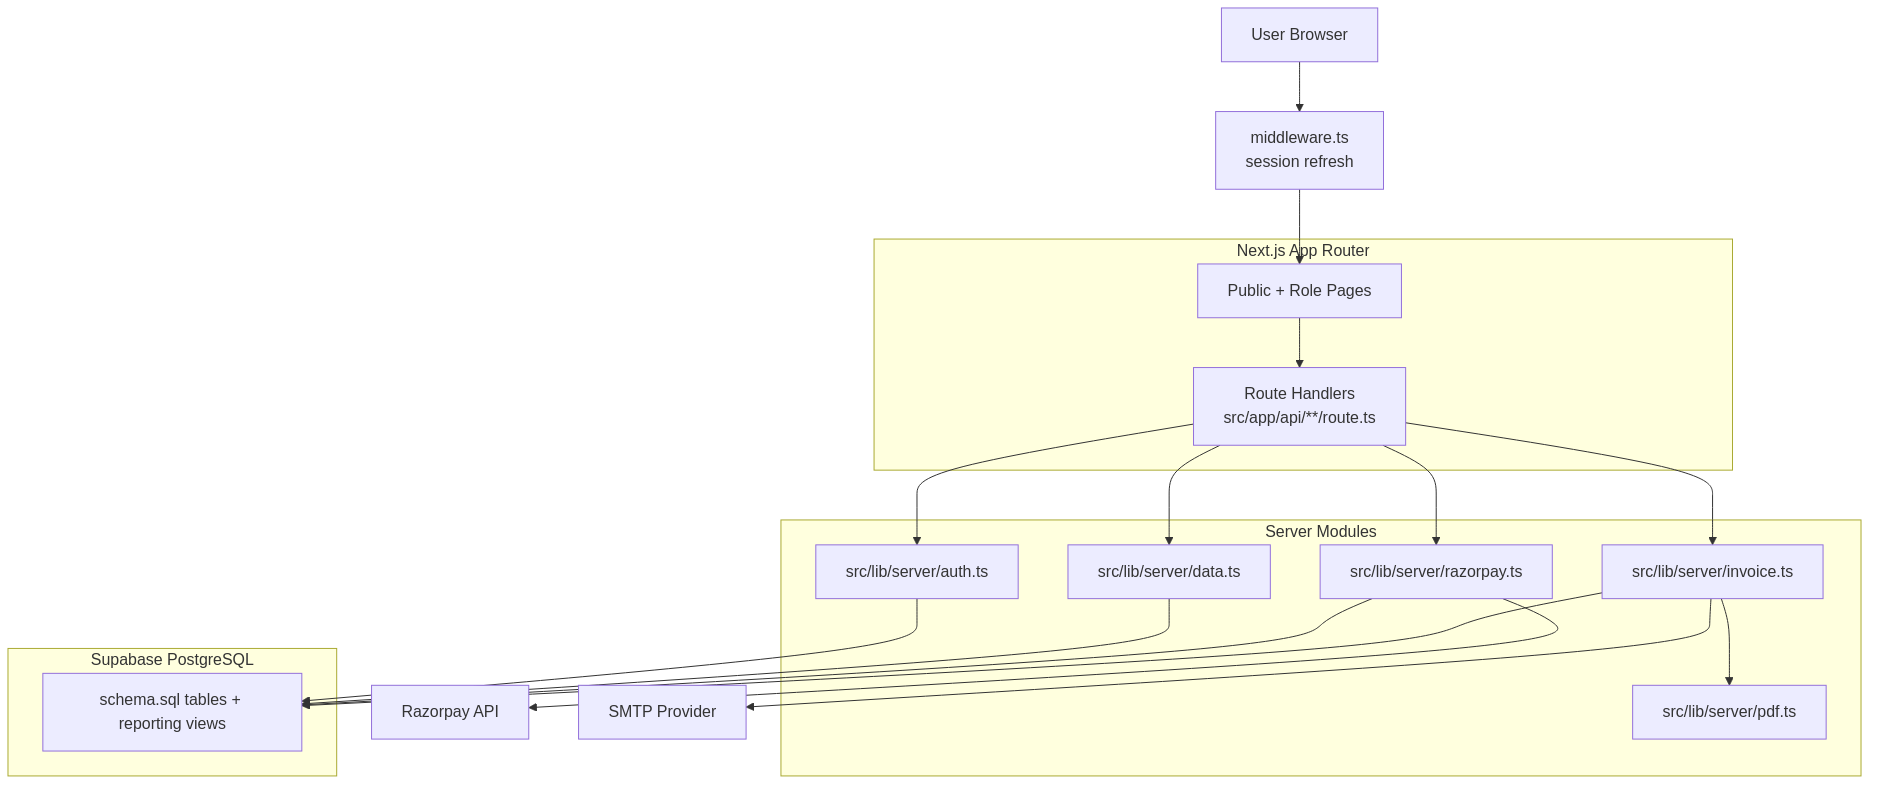
\includegraphics[width=\textwidth,height=0.8\textheight,keepaspectratio]{assets/system_architecture.png}
  \caption{System architecture derived from current code modules and integrations.}
\end{figure}

\begin{figure}[H]
  \centering
  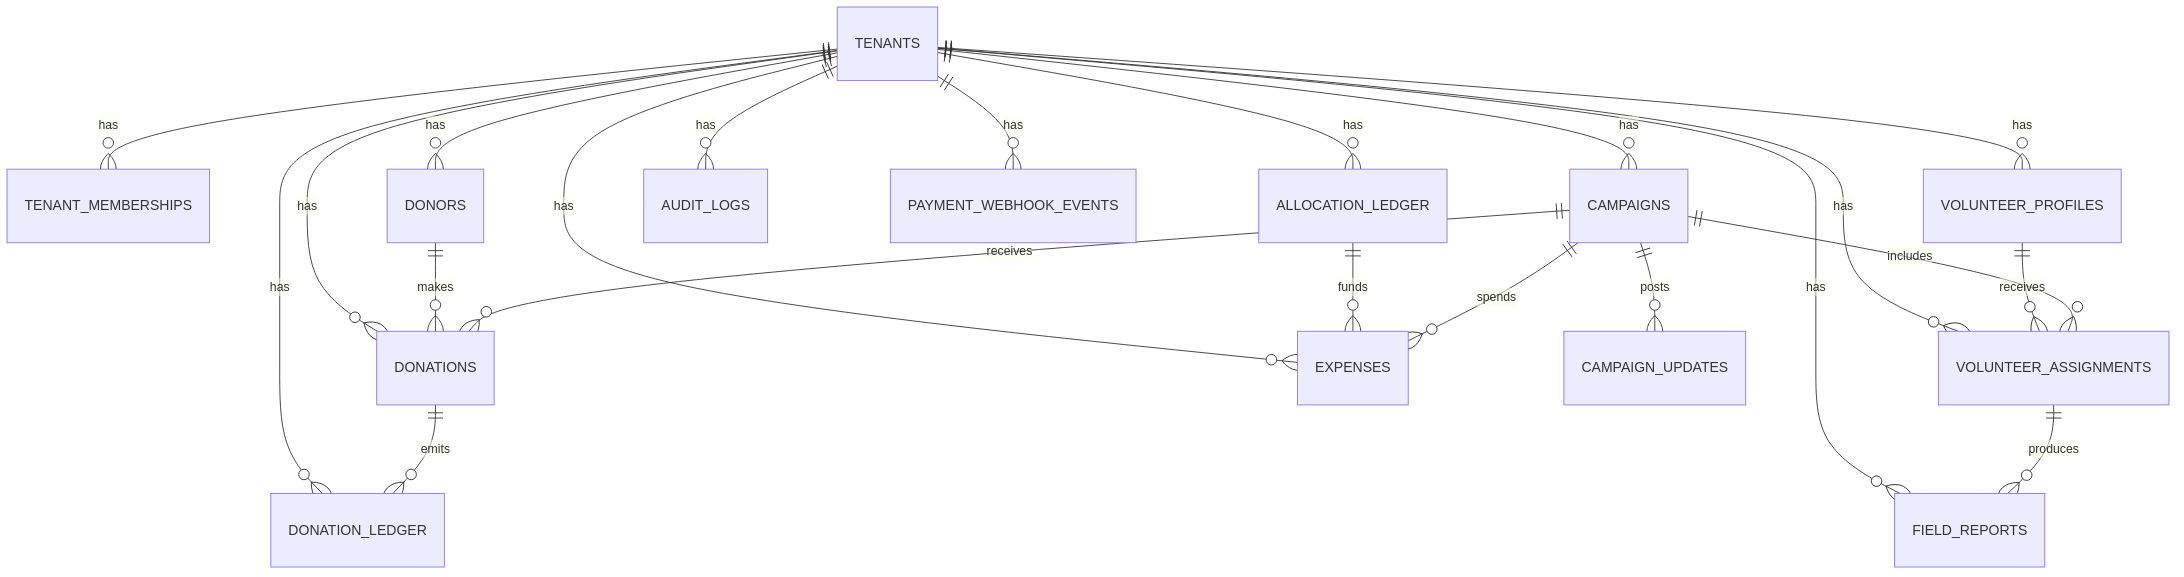
\includegraphics[width=\textwidth,height=0.8\textheight,keepaspectratio]{assets/er_diagram.png}
  \caption{Entity-relationship overview from \texttt{supabase/schema.sql}.}
\end{figure}

\begin{figure}[H]
  \centering
  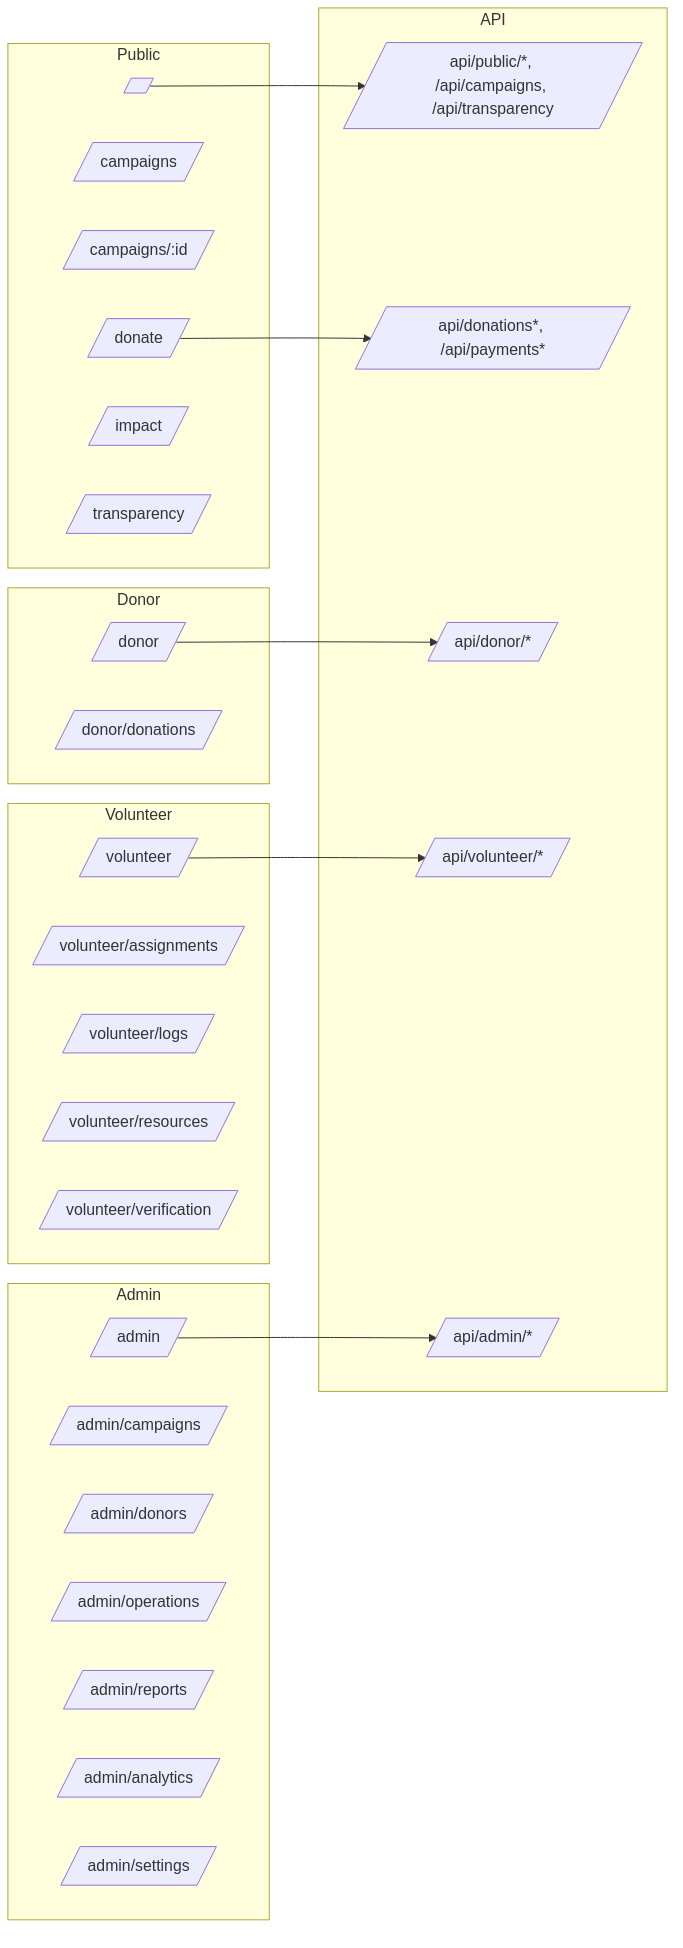
\includegraphics[width=\textwidth,height=0.8\textheight,keepaspectratio]{assets/route_map.png}
  \caption{Route and API map for public and role-scoped modules.}
\end{figure}

\begin{figure}[H]
  \centering
  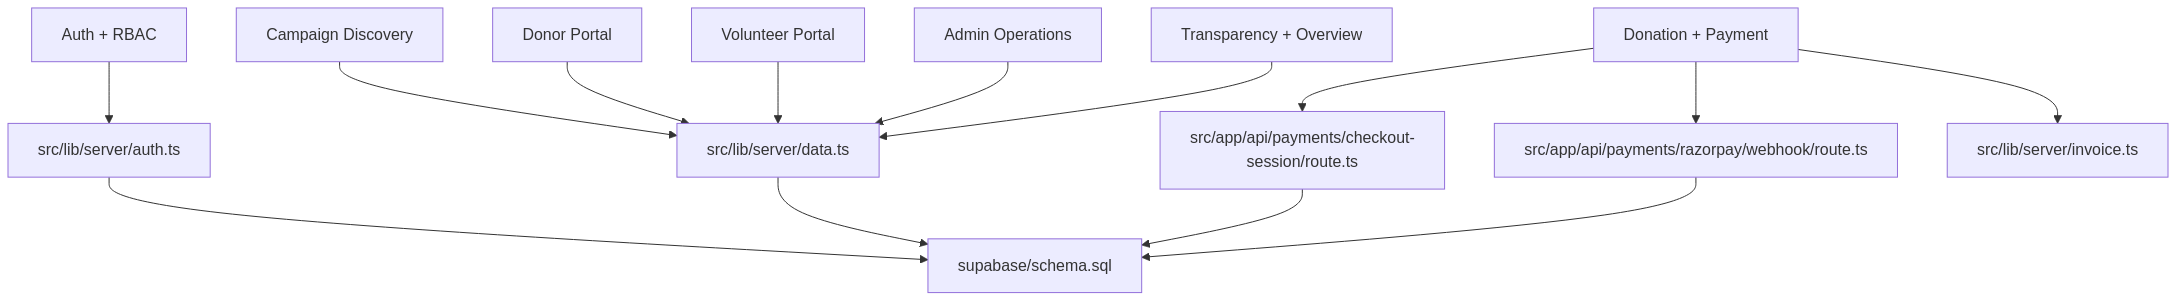
\includegraphics[width=\textwidth,height=0.8\textheight,keepaspectratio]{assets/feature_module_map.png}
  \caption{Feature-to-module map showing service and schema dependencies.}
\end{figure}

\begin{figure}[H]
  \centering
  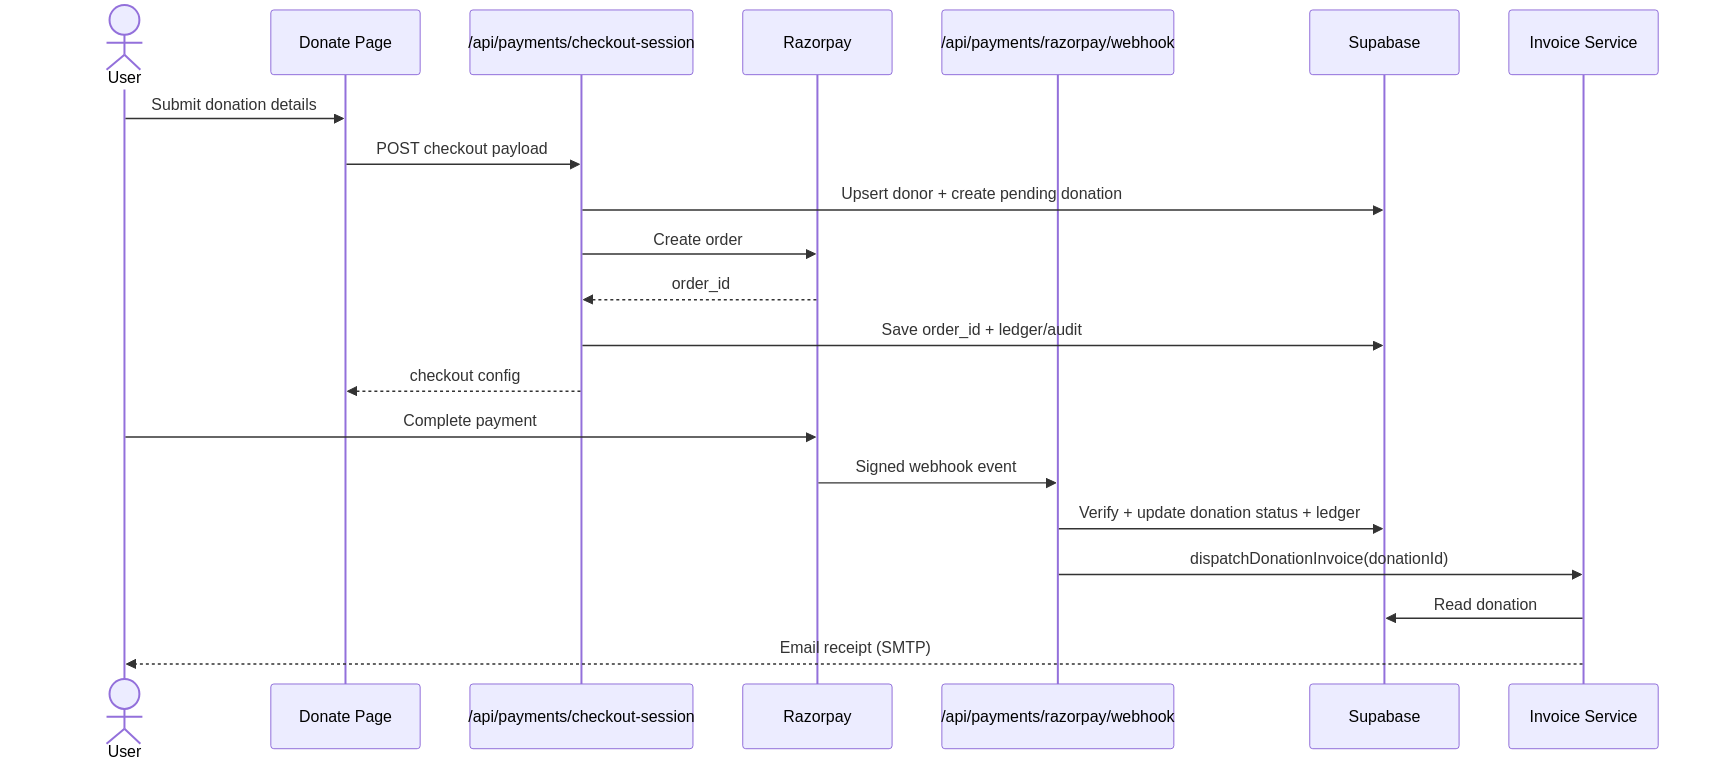
\includegraphics[width=\textwidth,height=0.8\textheight,keepaspectratio]{assets/donation_sequence.png}
  \caption{Donation flow sequence: checkout, payment confirmation, and receipt dispatch.}
\end{figure}

\section{Methodology (Evidence-First Documentation)}
This corrected report does not assert historical sprint metrics or stakeholder-process details unless directly evidenced in repository artifacts. The methodology here is implementation-first:
\begin{enumerate}
  \item identify claims in the previous document;
  \item map each claim to code evidence or mark as unsupported;
  \item rewrite sections from implemented modules and schemas;
  \item regenerate architecture and data diagrams from code-grounded structures.
\end{enumerate}

\section{Requirements (Code-Backed)}
\subsection{Functional requirements}
Derived from concrete routes and handlers:
\begin{itemize}
  \item role-based access to donor, volunteer, and admin modules;
  \item campaign discovery and detail retrieval;
  \item donation creation and status tracking;
  \item payment reconciliation via signed webhook processing;
  \item ledger and audit event capture;
  \item volunteer assignment/report workflows;
  \item admin operations, reporting, and analytics endpoints.
\end{itemize}

\subsection{Operational requirements}
\begin{itemize}
  \item Supabase and application environment variables for auth and tenancy;
  \item Razorpay API keys and webhook secret for payment workflows;
  \item SMTP configuration for invoice email dispatch.
\end{itemize}

\section{Implementation Notes}
\begin{itemize}
  \item Middleware: \texttt{middleware.ts} delegates session update handling.
  \item Auth context and role checks: \texttt{src/lib/server/auth.ts}.
  \item Data aggregation and role-specific data loaders: \texttt{src/lib/server/data.ts}.
  \item Payment path:
  \begin{itemize}
    \item checkout order creation: \texttt{/api/payments/checkout-session};
    \item webhook reconciliation: \texttt{/api/payments/razorpay/webhook};
    \item signature verification helper: \texttt{src/lib/server/razorpay.ts}.
  \end{itemize}
  \item Invoice path:
  \begin{itemize}
    \item dispatch: \texttt{src/lib/server/invoice.ts};
    \item PDF creation: \texttt{src/lib/server/pdf.ts}.
  \end{itemize}
\end{itemize}

\section{Results and Impact (Conservative Restatement)}
The corrected document limits results statements to repository-verifiable signals:
\begin{itemize}
  \item implemented route coverage across public and role-scoped modules;
  \item structured relational schema with audit and ledger tables;
  \item integrated payment and receipt pipeline with webhook persistence;
  \item available integration test suite for DB-backed API paths.
\end{itemize}

Where prior draft claims provided fixed performance/uptime/social-impact values without reproducible in-repo evidence, those claims are intentionally omitted or reframed.

\section{Reproducibility}
Diagram sources are maintained as Mermaid files in \texttt{report/diagrams/*.mmd}. Render with:
\begin{verbatim}
./report/render_diagrams.sh
\end{verbatim}

Compile this report from repository root:
\begin{verbatim}
pdflatex -output-directory report report/impactledger_corrected.tex
\end{verbatim}

\section*{Appendix: Source Index}
\begin{itemize}
  \item \texttt{report/claim\_mismatch\_matrix.csv}
  \item \texttt{report/canonical\_inventory.md}
  \item \texttt{report/diagrams/*.mmd}
  \item \texttt{supabase/schema.sql}
  \item \texttt{supabase/migrations/20260415\_add\_reporting\_views.sql}
  \item \texttt{src/lib/server/auth.ts}
  \item \texttt{src/lib/server/data.ts}
  \item \texttt{src/lib/server/razorpay.ts}
  \item \texttt{src/lib/server/invoice.ts}
  \item \texttt{src/lib/server/pdf.ts}
  \item \texttt{src/app/api/**/route.ts}
\end{itemize}

\end{document}
